\documentclass[a4paper,12pt]{report}

\usepackage{tabularx}
\usepackage{alltt, fancyvrb, url}
\usepackage{graphicx}
\usepackage[utf8]{inputenc}
\usepackage{float}
\usepackage{hyperref}
\usepackage{caption}


% Questo commentalo se vuoi scrivere in inglese.
\usepackage[italian]{babel}

\usepackage[italian]{cleveref}

% Centra verticalmente i contenuti delle righe
\renewcommand\tabularxcolumn[1]{m{#1}}


\title{\textbf{Elaborato per il corso Basi di dati}
Progettazione di una base di dati per la gestione di video perizie}


\author{
\\Buizo Manuel
\\Matteini Mattia
\\Paganelli Alberto
}
\date{\today}


\begin{document}

\maketitle

\tableofcontents

\chapter{Analisi dei requisiti}

Si vuole realizzare un database a supporto della gestione di video perizie (perizie a distanza tramite videochiamata) effettuate per varie assicurazioni italiane.
\\
La base di dati dovrà immagazzinare informazioni relative alle assicurazioni, ai sinistri, agli assicurati, agli studi peritali e ai relativi periti.
\\
Tutte le assicurazioni devono avere la possibilità di controllare documenti e dati delle video-perizie effettuate.


\section{Intervista }

Si vuole tenere traccia di tutte le video-perizie effettuate, di ogni studio peritale e delle parti coinvolte. 
\\
Ogni assicurazione dovrà generare sinistri di varia natura (R.C.A., Furto, Incendio, ecc…).
\\
Questi verranno assegnati agli studi, i quali si occuperanno di portare a termine le attività peritali.
\\
Ogni studio peritale dispone di un supervisore che avrà il compito di ricevere i sinistri che arrivano dalle assicurazioni e di smistarli ai periti del proprio studio.
\\
Il supervisore dello studio quindi creerà un incarico relativo al sinistro arrivatogli e lo assegnerà ad un perito che dovrà svolgere le attività peritali inerenti (video-perizia, richiesta documenti, ecc.. ).
\\
Ogni incarico conterrà informazioni riguardanti sinistro di riferimento, perito incaricato e stato di avanzamento (Aperto, Svolgimento, Chiuso).
\\
Inoltre includerà uno storico delle video-perizie svolte e  l’insieme dei documenti richiesti all’assicurato (come eventuali contratti o documenti personali).
\\
Il perito quando riceverà l'incarico dal supervisore, dovrà mettersi in contatto con l'assicurato al fine di definire i dettagli per l'effettuazione della video-perizia ed eventualmente richiedere dei documenti per le pratiche preliminari.
\\
Durante una video-perizia si potranno raccogliere vari media (foto e video) che saranno allegati alla perizia.
\\
Ogni media a sua volta è comprensivo di metadati ricavati dal GPS del dispositivo dell’assicurato.
\\
Per ogni documento invece dovremo sapere la sua tipologia e se sarà necessaria o meno la firma dell’assicurato.
\\
In questo modo teniamo traccia di ogni sinistro, dall’assicurazione ai tipi di documenti richiesti o alle foto georeferenziate scattate durante la video-perizia.


\section{Definizione delle specifiche in linguaggio naturale ed estrazione dei concetti principali}
\subsection{Glossario dei termini}
\mbox{}\\
\def\arraystretch{2}% 
\begin{tabularx}{\textwidth}{ m{3cm} | m{6cm} | m{3cm}}
    \textbf{Termine} & \textbf{Descrizione} & \textbf{Sinonimo} \\
\hline
Assicurazione & Colei che riceve da cittadini nuove richieste e crea sinistri & Ente esterno\\ \hline
Studio & Colei che riceve da cittadini nuove richieste e crea sinistri & Ente esterno\\ \hline
Supervisore & Colui che, all’interno dello studio, ha il compito di generare incarichi e assegnarli ad uno dei propri periti & Coordinatore\\ \hline
Perito & Colui che si occupa della attività peritali & Incaricato dal supervisore, membro dello studio/ufficio\\ \hline
Assicurato & Colui che farà parte alla video-perizia e che si occupa della ripresa del sinistro & Cliente, parte coinvolta\\ \hline
Sinistro & Danno e relativo tipo di danno da periziare & \\ \hline
Incarico & Insieme di attività peritali atte all’intero svolgimento della perizia & Fascicolo\\ \hline
Video-perizia & Perizia eseguita telematicamente tramite smartphone o dispositivo mobile & Perizia telematica, videochiamata
\\ 

\end{tabularx}
\noindent
\def\arraystretch{2}% 
\begin{tabularx}{\textwidth}{ m{3cm} | m{6cm} | m{3cm}}
Documenti & Documenti richiesti al fine di eseguire una perizia completa & \\ \hline
Media & Media raccolti durante la video-perizia, comprensivi di metadati & Foto, video\\ \hline
Metadati & Informazioni raccolte dal dispositivo dell’assicurato, in questo caso specifico quelli relativi alla geolocalizzazione & \\
\end{tabularx}
\\
\\

\subsection{Riassunto dei concetti principali}

Ogni Sinistro, è individuato tramite un identificativo incrementale e può essere di un solo \texttt{TIPO\_SINISTRO}.
\\
Un’ Assicurazione, identificata tramite la sua denominazione, cede la gestione del \texttt{SINISTRO} allo \texttt{STUDIO} (identificato dalla P.Iva e da un identificativo incrementale) e lo stesso sinistro non può essere assegnato ad un altro ufficio.
\\
Ogni studio può avere più di un \texttt{SUPERVISORE} ma ne ha almeno uno.
\\
Gli \texttt{STUDI} possono ricevere sinistri da tutte le \texttt{ASSICURAZIONI} e un \texttt{SUPERVISORE} deve  creare un \texttt{INCARICO} e assegnarne la gestione ad un proprio \texttt{PERITO}.
\\
Non può essere assegnato un \texttt{INCARICO} a più di un \texttt{PERITO} ma a un \texttt{PERITO} possono essere assegnati più \texttt{INCARICHI} e da più \texttt{SUPERVISORI}.
\\
Il \texttt{PERITO}, che avrà il compito di svolgere le attività peritali inerenti all’\texttt{INCARICO} a lui assegnato, dovrà poter svolgere anche più di una \texttt{VIDEO-PERIZIA} per entrare in contatto con l’\texttt{ASSICURATO} e poter scrivere una descrizione del danno (ad esempio se si vede meglio in altra fase della giornata, danno grande che richiede più videochiamate, ecc...  ).
\\
Potrà anche lavorare a più \texttt{INCARICHI} alla volta e nello stesso giorno.
\\
L’\texttt{ASSICURATO} invece sarà registrato tramite un’anagrafica ed identificato mediante il codice fiscale.
\\
La \texttt{VIDEO-PERIZIA} e i \texttt{MEDIA} raccolti, sono relativi esclusivamente ad un \texttt{INCARICO}. 
\\
Ogni \texttt{INCARICO} possiede anche una raccolta di \texttt{DOCUMENTI} riguardanti il sinistro.
\\
I \texttt{DOCUMENTI} riguardano principalmente l’assicurato e il tipo di sinistro, non sapendo quindi quanti documenti possono essere richiesti, non vi è nessun vincolo. 
\\
Ogni \texttt{VIDEO-PERIZIA} deve comprendere anche un luogo effettivo e sarà quindi localizzato tramite coordinate e sistema di riferimento. (Altitudine, Latitudine, Longitudine e Est o Ovest).
\\
Ogni \texttt{VIDEO-PERIZIA} ed ogni \texttt{MEDIA} deve essere localizzato per essere definita valida.
\\
\\
\textbf{Segue un elenco delle principali azioni richieste:}
\begin{enumerate}
    \item \textsc{Registrare/eliminare assicurazioni}
    \item \textsc{Registrare/eliminare un assicurato}
    \item \textsc{Erogazione di una nuova polizza da parte di un assicurazione}
    \item \textsc{Registrare/eliminare studi peritali}
    \item \textsc{Assumere/licenziare un nuovo perito o dirigente in uno studio}
    \item \textsc{QUALCOSA SU TEAM????}
    \item \textsc{Stipulare un nuovo contratto tra assicurato e assicurazione}
    \item \textsc{Creare nuovo lavoro e assegnarlo a un perito}
    \item \textsc{Creare l’incarico da svolgere in base al lavoro di un perito}
    \item \textsc{Aggiornare lo stato di un incarico}
    \item \textsc{Leggere tutti gli incarichi aperti in un determinato studio}
    \item \textsc{Aggiungere dei documenti ad un incarico}
    \item \textsc{Inserire una video-perizia per un incarico}
    \item \textsc{Allegare i media raccolti alla video-perizia}
    \item \textsc{Raccogliere tutte le informazioni relative a un incarico (incluse video-perizie e documenti)}
\end{enumerate}


\chapter{Progettazione Concettuale}

\section{Schema scheletro}

\textsc{Seguiranno ora dei sotto-schemi E/R iniziali, che verranno raffinati nella sezione successiva}


\clearpage
Dal dominio identificato in seguito all’intervista si può notare che sono presenti tre entità rappresentanti delle persone: \textbf{Perito}, \textbf{Supervisore} e \textbf{Assicurato}.
\\
Queste entità quindi sono generalizzate da \textbf{Persona}, che raccoglie gli attributi in comune.
\\
In seguito si ha una collaborazione tra \textbf{Studi Peritali} e \textbf{Assicurazioni}, uno studio può non avere ancora collaborazioni con le assicurazioni (perché magari creato da poco) e può averne molteplici, invece un’ssicurazione deve collaborare con almeno uno studio perché altrimenti non potrebbe lavorare e non avrebbe senso di esistere in questa modellazione.
\\
Le assicurazioni sono identificate dalle proprie denominazioni, mentre gli studi da un ID. 
%poiché è difficile distinguerle per sedi o per partite IVA (una singola P. IVA ) potrebbe avere più studi.
\\
Uno studio peritale può assumere sia supervisori (almeno uno altrimenti nessuno smisterebbe gli incarichi) sia periti, abbiamo quindi un associazione ternaria che andremo a rifinire in seguito.
\\
\begin{figure}[ht]
    \begin{center}
        \centering
        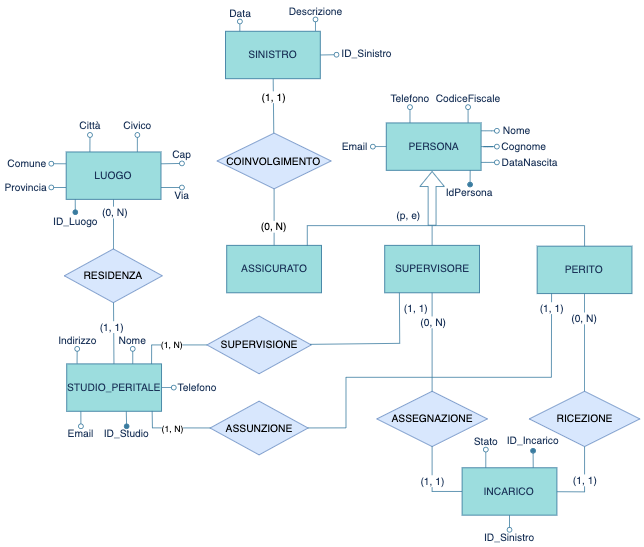
\includegraphics[width=\textwidth]{img/StudioPeritale.png}
    \end{center}
\end{figure}
\clearpage

Un \textbf{Perito}, in un determinato momento, può svolgere zero incarichi, ma anche molteplici, invece un \textbf{Incarico} può essere svolto solo da un perito.
\\
L’incarico deve per forza avere almeno una \textbf{Video Perizia} annessa (per la corretta esecuzione delle pratiche peritali), inoltre è identificato dalla combinazione di codice e perito.
\\
La video perizia può essere eseguita solo in presenza di un incarico, e quindi è identificata da un numero incrementale combinato al codice dell’incarico corrispondente.
\\
Durante la videochiamata possono essere scattate \textbf{Foto} e registrati \textbf{Video}, ma non è sempre necessario.
\\
Questi ultimi sono entità figlie di \textbf{Media}, hanno una dimensione e sono identificati dal nome e dall’estensione del file.
\\
\begin{figure}[ht]
    \begin{center}
        \centering
        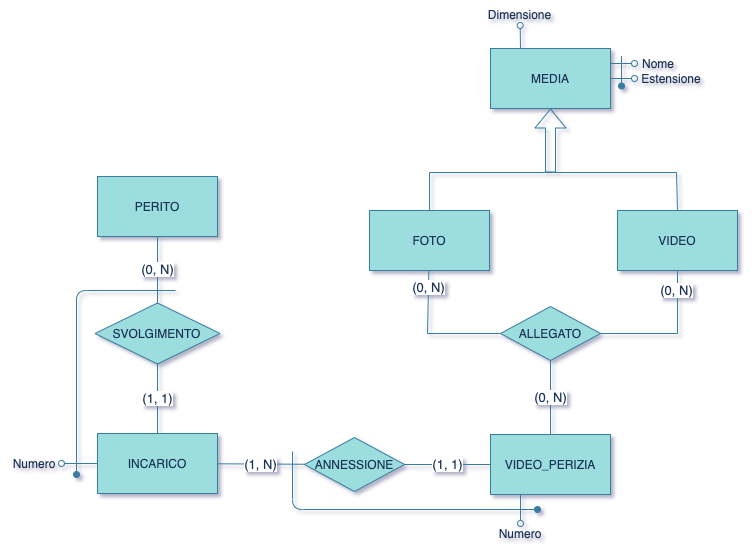
\includegraphics[width=\textwidth]{img/VideoPerizia.png}
    \end{center}
\end{figure}
\clearpage

\section{Raffinamenti proposti}

È assolutamente inutile, ed è anzi controproducente, descrivere classe-per-classe (o peggio ancora metodo-per-metodo) com'è fatto il vostro software: è un livello di dettaglio proprio della documentazione dell'API (deducibile dalla Javadoc).

\textbf{È necessario che ciascun membro del gruppo abbia una propria sezione di design dettagliato,
di cui sarà il solo responsabile}.
Per continuare il parallelo con la vettura di Formula 1, se nei fogli di progetto che mostrano il
design delle sospensioni anteriori appaiono pezzi che appartengono al volante o al turbo, c'è una
chiara indicazione di qualche problema di design.

Si divida la sezione in sottosezioni, e per ogni aspetto di design che si vuole approfondire, si presenti:
\begin{enumerate}
    \item: una breve descrizione in linguaggio naturale del problema che si vuole risolvere, se necessario ci si può aiutare con schemi o immagini;
    \item: una descrizione della soluzione proposta, analizzando eventuali alternative che sono state prese in considerazione, e che descriva pro e contro della scelta fatta;
    \item: uno schema UML che aiuti a comprendere la soluzione sopra descritta;
    \item: se la soluzione è stata realizzata utilizzando uno o più pattern noti, si spieghi come questi sono reificati nel progetto
    (ad esempio: nel caso di Template Method, qual è il metodo template;
    nel caso di Strategy, quale interfaccia del progetto rappresenta la strategia, e quali sono le sue implementazioni;
    nel caso di Decorator, qual è la classe astratta che fa da Decorator e quali sono le sue implementazioni concrete; eccetera);
\end{enumerate}
%
La presenza di pattern di progettazione \emph{correttamente utilizzati} è valutata molto positivamente.
%
L'uso inappropriato è invece valutato negativamente: a tal proposito, si raccomanda di porre particolare attenzione all'abuso di Singleton, che, se usato in modo inappropriato, è di fatto un anti-pattern.

\section{Schema concettuale finale}

\paragraph{Problema} GLaDOS ha più personalità intercambiabili, la cui presenza deve essere trasparente al client.

\paragraph{Soluzione} Il sistema per la gestione della personalità utilizza il \textit{pattern Strategy}, come da
\Cref{img:strategy}: le implementazioni di \texttt{Personality} possono essere modificate, e la
modifica impatta direttamente sul comportamento di GLaDOS.

\begin{figure}[H]
\centering{}
\includegraphics[width=.7\textwidth]{img/observer}
\caption{Il pattern Observer è usato per consentire a GLaDOS di informare tutti i sistemi di output in ascolto}
\label{img:observer}
\end{figure}



\begin{figure}[h]
\centering{}
\includegraphics[width=\textwidth]{img/badarch}
\caption{Schema UML mal fatto e con una pessima descrizione, che non aiuta a capire. Don't try this at home.}
\label{img:badarch}
\end{figure}


\chapter{Progettazione Logica}
\section{Stima del volume dei dati}

\mbox{}\\
\def\arraystretch{2}% 
\begin{tabularx}{\textwidth}{ p{6cm} | >{\centering\arraybackslash}p{2cm} | >{\centering\arraybackslash}X }
    \textbf{Concetto} & \textbf{Costrutto} & \textbf{Volume} \\
\hline
ASSICURAZIONE & E & 30\\ \hline
POLIZZA & E & 2.000.000\\ \hline
ASSICURATO & E & 1.000.000\\ \hline
EROGAZIONE & A & 300\\ \hline
STIPULAZIONE & A & 2.000.000\\ \hline
GENERAZIONE & A & 100.000\\ \hline
SINISTRO & E & 100.000\\ \hline
DELEGAZIONE & A & 100.000 \\ \hline
STUDIO\_PERITALE & E & 3.000\\ \hline
SPECIFICAZIONE & A & 100.000\\ \hline
CATEGORIA\_SINISTRO & E & 20\\
\end{tabularx}

\noindent
\def\arraystretch{2}% 
\begin{tabularx}{\textwidth}{ p{6cm} | >{\centering\arraybackslash}p{2cm} | >{\centering\arraybackslash}X }
DIRIGENTE & E & 4.000\\ \hline
DIREZIONE & A & 4.000\\ \hline
PERITO & E & 60.000\\ \hline
ASSUNZIONE & A & 60.000\\ \hline
ASSEGNAZIONE & E & 80.000\\ \hline
RICEZIONE & A & 80.000\\ \hline
LAVORO & A & 80.000\\
\end{tabularx}
\\
\\
\\
\\
\\
\noindent
\def\arraystretch{2}% 
\begin{tabularx}{\textwidth}{ p{6cm} | >{\centering\arraybackslash}p{2cm} | >{\centering\arraybackslash}X }
SVOLGIMENTO & A & 100.000\\ \hline
INCARICO & E & 100.000\\ \hline
FASCICOLO & A & 100.000\\ \hline
DOCUMENTI & E & 300.000\\ \hline
ANNESSIONE & A & 120.000\\ \hline
VIDEO\_PERIZIA & E & 120.000\\ \hline
ALLEGATO & A & 50.000\\ \hline
MEDIA & E & 70.000\\
\end{tabularx}

\clearpage
\section{Descrizione delle operazioni principali e stima della loro frequenza}

\def\arraystretch{2}% 
\begin{tabularx}{\textwidth}{ >{\centering\arraybackslash}p{2cm} | X |  >{\centering\arraybackslash}p{3cm} }
    \textbf{Codice} & \textbf{Operazione} & \textbf{Frequenza}\\
\hline
1 & Registrare/eliminare assicurazioni & 1 al mese\\ \hline
2 & Registrare/eliminare un assicurato & 500 al giorno\\ \hline
3 & Erogazione di una nuova polizza da parte di un assicurazione & 75 all'anno\\ \hline
4 & Registrare/eliminare studi peritali & 50 al mese\\ \hline
5 & Assumere/licenziare un nuovo perito o dirigente in uno studio & 50.000 al mese\\ \hline
6 & QUALCOSA SU TEAM???? & E\\ \hline
7 & Stipulare un nuovo contratto tra assicurato e assicurazione & 1.000 al giorno\\ \hline
8 & Creare nuovo lavoro e assegnarlo a un perito & 25.000 al giorno\\ \hline
9 & Creare l’incarico da svolgere in base al lavoro di un perito & 25.000 al giorno\\ \hline
10 & Aggiornare lo stato di un incarico & 50.000 al giorno\\
\end{tabularx}

\noindent
\def\arraystretch{2}% 
\begin{tabularx}{\textwidth}{ >{\centering\arraybackslash}p{2cm} | X |  >{\centering\arraybackslash}p{3cm} }
11 & Leggere tutti gli incarichi aperti in un determinato studio & 2.000 al giorno\\ \hline
12 & Aggiungere dei documenti ad un incarico & 35.000 al giorno\\ \hline
13 & Inserire una video-perizia per un incarico & 30.000 al giorno\\ \hline
14 & Allegare i media raccolti alla video-perizia & 20.000 al giorno\\ \hline
15 & Raccogliere tutte le informazioni relative a un incarico (incluse video-perizie e documenti) & 8.000 al giorno\\
\end{tabularx}
\\
\\
\section{Schemi di navigazione e tabelle degli accessi}

\subsection{1 - Registrare/eliminare assicurazioni}

\def\arraystretch{2}% 
\begin{tabularx}{\textwidth}{ >{\centering\arraybackslash}p{3cm} | >{\centering\arraybackslash}p{2cm} | >{\centering\arraybackslash}X |  >{\centering\arraybackslash}p{2cm} }
    \textbf{Concetto} & \textbf{Costrutto} & \textbf{Accessi} & \textbf{Tipo} \\
\hline
Assicurazione & E & 1 & S \\
\end{tabularx}
\begin{center}
\textbf{Totale : 1S * 1 al giorno = 2 al giorno}
\end{center}

\subsection{2 - Registrare/eliminare un assicurato}

\def\arraystretch{2}% 
\begin{tabularx}{\textwidth}{ >{\centering\arraybackslash}p{3cm} | >{\centering\arraybackslash}p{2cm} | >{\centering\arraybackslash}X |  >{\centering\arraybackslash}p{2cm} }
    \textbf{Concetto} & \textbf{Costrutto} & \textbf{Accessi} & \textbf{Tipo} \\
\hline
Assicurato & E & 1 & S \\
Stipulazione & E & 1 & S \\
Polizza & E & 1 & S \\
Erogazione & E & 1 & S \\
\end{tabularx}
\begin{center}
\textbf{Totale : 4S * 500 al giorno = 4.000 al giorno}
\end{center}

\subsection{3 - Erogazione di una nuova polizza da parte di un assicurazione}

\def\arraystretch{2}% 
\begin{tabularx}{\textwidth}{ >{\centering\arraybackslash}p{3cm} | >{\centering\arraybackslash}p{2cm} | >{\centering\arraybackslash}X |  >{\centering\arraybackslash}p{2cm} }
    \textbf{Concetto} & \textbf{Costrutto} & \textbf{Accessi} & \textbf{Tipo} \\
\hline
Assicurato & E & 1 & S \\
Stipulazione & E & 1 & S \\
Polizza & E & 1 & S \\
Erogazione & E & 1 & S \\
\end{tabularx}
\begin{center}
\textbf{Totale : 4S * 500 al giorno = 4.000 al giorno}
\end{center}

%3 & Erogazione di una nuova polizza da parte di un assicurazione & 75 all'anno\\ \hline

\section{Raffinamento dello schema}

Questa sezione, come quella riguardante il design dettagliato va svolta \textbf{singolarmente da ogni membro del gruppo}.


\section{Analisi delle ridondanze}

Questa sezione, come quella riguardante il design dettagliato va svolta \textbf{singolarmente da ogni membro del gruppo}.


\section{Traduzione di entità e associazioni in relazioni}

Questa sezione, come quella riguardante il design dettagliato va svolta \textbf{singolarmente da ogni membro del gruppo}.


\section{Schema relazionale finale}

Questa sezione, come quella riguardante il design dettagliato va svolta \textbf{singolarmente da ogni membro del gruppo}.


\section{Traduzione delle operazioni in query SQL}

Questa sezione, come quella riguardante il design dettagliato va svolta \textbf{singolarmente da ogni membro del gruppo}.



\chapter{Progettazione dell'applicazione}

In quest'ultimo capitolo si tirano le somme del lavoro svolto e si delineano eventuali sviluppi
futuri.

\textit{Nessuna delle informazioni incluse in questo capitolo verrà utilizzata per formulare la valutazione finale}, a meno che non sia assente o manchino delle sezioni obbligatorie.
%
Al fine di evitare pregiudizi involontari, l'intero capitolo verrà letto dai docenti solo dopo aver formulato la valutazione.

\section{Autovalutazione e lavori futuri}

\textbf{È richiesta una sezione per ciascun membro del gruppo, obbligatoriamente}.
%
Ciascuno dovrà autovalutare il proprio lavoro, elencando i punti di forza e di debolezza in quanto prodotto.
Si dovrà anche cercare di descrivere \emph{in modo quanto più obiettivo possibile} il proprio ruolo all'interno del gruppo.
Si ricorda, a tal proposito, che ciascuno studente è responsabile solo della propria sezione: non è un problema se ci sono opinioni contrastanti, a patto che rispecchino effettivamente l'opinione di chi le scrive.
Nel caso in cui si pensasse di portare avanti il progetto, ad esempio perché effettivamente impiegato, o perché sufficientemente ben riuscito da poter esser usato come dimostrazione di esser capaci progettisti, si descriva brevemente verso che direzione portarlo.

\section{Difficoltà incontrate e commenti per i docenti}

Questa sezione, \textbf{opzionale}, può essere utilizzata per segnalare ai docenti eventuali problemi o difficoltà incontrate nel corso o nello svolgimento del progetto, può essere vista come una seconda possibilità di valutare il corso (dopo quella offerta dalle rilevazioni della didattica) avendo anche conoscenza delle modalità e delle difficoltà collegate all'esame, cosa impossibile da fare usando le valutazioni in aula per ovvie ragioni.
%
È possibile che alcuni dei commenti forniti vengano utilizzati per migliorare il corso in futuro: sebbene non andrà a vostro beneficio, potreste fare un favore ai vostri futuri colleghi.
%
Ovviamente \textit{il contenuto della sezione non impatterà il voto finale}.




\end{document}
